\documentclass{TDP005mall}



\newcommand{\version}{Version 0.1}
\author{Hadi Ansari, \url{hadan326@student.liu.se}\\
  Nils Bark, \url{nilba048@student.liu.se}}
\title{Kravspecifikation}
\date{2020-11-22}
\rhead{Hadi Ansari\\
Nils Bark}



\begin{document}
\projectpage
\tableofcontents
\thispagestyle{empty}
\cleardoublepage

\section{Revisionshistorik}
\begin{table}[!h]
\begin{tabularx}{\linewidth}{|l|X|l|}
\hline
Ver. & Revisionsbeskrivning & Datum \\\hline
0.1 & Första utkastet & 2020-11-17 \\\hline
1.0 & Komplettering efter feed-back& 2020-11-22 \\\hline

\end{tabularx}
\end{table}


\section{Spelidé}
Spelet går ut på att spelaren, via sitt flygplan, ska flyga igenom banor där den möter andra fiendeplan och bomber som försöker hindra en på vägen mot slutet. 
Målet är att samla så många poäng som möjligt genom att skjuta och förstöra så många fiender som möjligt samtidigt som spelaren undviker att själv bli träffad av fienderna eller deras skott.
Det kommer även finnas power-ups att plocka upp i varje nivå. Dessa ger diverse positiva effekter som hjälper spelaren med sitt mål. Ju skickligare spelaren är på att samla ihop poäng, desto fler stjärnor får den i slutet av varje nivå

Spelet utspelar sig i en 2D-miljö från ett sidoperspektiv. Spelaren kan röra sig i åtta olika
riktningar och skjuta skott mot de ankommande fienderna. Skotten som spelaren skjuter gör
skada till fienderna om den träffar och kommer till slut förstöra den. När en fiende förstörs
får spelaren en visst antal poäng. Det kommer även då och då att dyka upp Power-ups från högra sidan av skärmen. 
Fienderna kommer att närma sig från höger om skärmen och röra sig mot vänster. 
Fiendertyperna kan även ha unika rörelsemönster när de färdas över skärmen. 
Fienderna gör skada till spelaren antigen genom att vidröra den
eller genom att träffa spelaren med sina skott (om de skjuter skott). 
Spelaren har ett antal liv som förloras allt eftersom den har blivit träffad av fienderna/deras skott.
När spelarens liv når noll avslutas nivån.

\section{Målgrupp}
Målgruppen är alla som tycker om utmanande skjut-spel i denna klassiska arkad-stil.

\section{Spelupplevelse}
Det roliga med spelet fås från en kombination av den ständigt ökande utmaningen och poänginsamlingen. Spelet kan spelas om och om igen för att få ett så bra poängrekord som möjligt.

\section{Spelmekanik}
Spelaren styrs av W, A, S, D eller piltangenterna. Spelaren skjuter med mellanslag.
\begin{table}[!h]
\begin{tabularx}{\linewidth}{|X|X|}
\hline
Tangentknapp & Åtgärd\\\hline
W & Flytta spelaren uppåt\\\hline
S & Flytta spelaren nedå\\\hline
A & Flytta spelaren vänster\\\hline
D & Flytta spelaren höger\\\hline
Mellanslag & Skjuta skott\\\hline

\end{tabularx}
\end{table}

\section{Regler}
Nedan beskrivs de olika regler som spelet använder sig av.
\subsection{Spelplan}
\begin{itemize}
\item Spelplanen har en fixerad storlek.
\item Spelaren kan endast befinna sig inom spelplanen medan fienderna kan komma in i spelplanen från sidorna. 
\item Objekt som åker ut ur spelplanen förstörs.
\end{itemize}

\subsection{Hastighet}
Alla typer av objekt på spelplanen har en egen hastighet. Denna hastighet rangordnas i detta dokument från 1 till 4, där 4 är snabbast.
Nivåerna är inte de faktiska tal som kommer att användas (hastighet 4 är inte nödvändigtvis dubbelt så snabbt som 2) 
utan används bara för att ge ett perspektiv kring hur de relaterar till varandra.

\subsection{Skott}
\begin{itemize}
\item Spelaren och fienderna skjuter samma typ av skott.
\item Ett skott gör 1 skada vid kollision med giltligt objekt.
\item Alla skott rör sig med hastighet 4.
\item De skadar motståndarens och minskar dens antal liv med 1.
\end{itemize}

\subsection{Spelare}
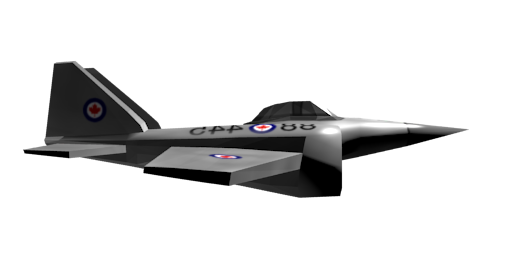
\includegraphics[scale=0.2]{Images/Player.png}
\begin{itemize}
\item Spelaren har en fixerad storlek.
\item Spelaren kan röra på sig i åtta riktningar.
\item Spelaren skjuter skott framåt som skadar fienderna när de kolliderar.
\item Hur ofta spelaren kan skjuta baseras på en timer mellan varje skott. 
\item Spelaren kan plocka upp power-ups genom att kollidera med dem.
\item Spelarens skott har ingen effekt på power-ups.
\item Spelaren har tre liv och kan inte gå över detta.
\item Spelaren kan få liv genom att plocka upp heal Power-ups.
\item Spelaren förlorar 1 liv när den kolliderar med skott.
\item När spelaren tar skada (via kollision med fiende eller dess skott) blir den odödlig i tre sekunder.
\item När spelarens liv når noll är spelet över.
\item Spelaren rör sig med hastighet 2.


\end{itemize}

\subsection{Fiende}
Fiender i spelet kommer att vara spelarens främsta hinder (och källa till poäng). 
Det finns tre typer av fiender som spelaren kommer att stöta på under spelets gång. 
Grupperingen och antalet fiender varierar från nivå till nivå. 
Alla fiender ignorerar kollision med varandras modeller, andra fienders skott, och power-ups. De kan därmed endast ta skada från spelaren. 
Nedan kommer allmänna regler som har tänkts följas i spelet.

\begin{itemize}
\item Fienderna kan röra på sig.
\item De olika fiendetyperna rör sig med olika hastigheter.
\item Fienderna rör sig enligt förbestämda mönster över skärmen.
\item Olika fiendetyper rör sig i olika mönster.
\item Fienderna skjuter skott enligt en bashastighet som spelaren.
\item Fiender skadar spelaren ifall de kolliderar med den.
\item Fiender förstörs när de kolliderar med spelaren.
\item Fiender har ett antal liv. 
\item När en fiendes liv når noll dör den.
\item Fiender kommer från högersidan av skärmen och de rör sig åt vänster enligt sitt mönster tills de når slutet av spelplanen.
\end{itemize}

De olika fiendetyperna i spelet har följande egenskaper:

\subsubsection*{Small plane}
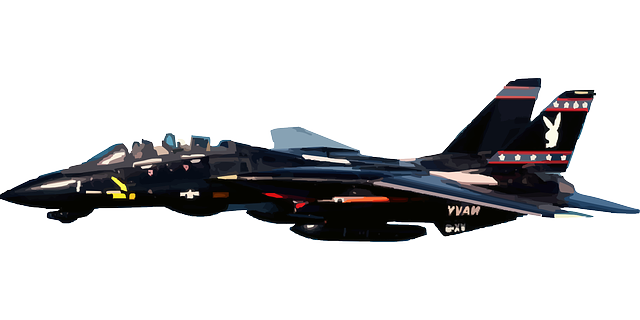
\includegraphics[scale=0.15]{Images/Enemy1.png}
\begin{itemize}
\item Den har samma (fixerade) storlek som spelaren.
\item Den har 1 liv.
\item Vid kollision skadar den spelaren med 1.
\item Den rör sig åt vänster enligt en bestämd våg-liknande rörelse (se figur 1).
\item Den har röreslehastighet 3. 
\item Den skjuter skott rakt fram.
\item Den skjuter skott när den är i höjd med spelaren.
\end{itemize}
\begin{figure}[h!]
  \centering
  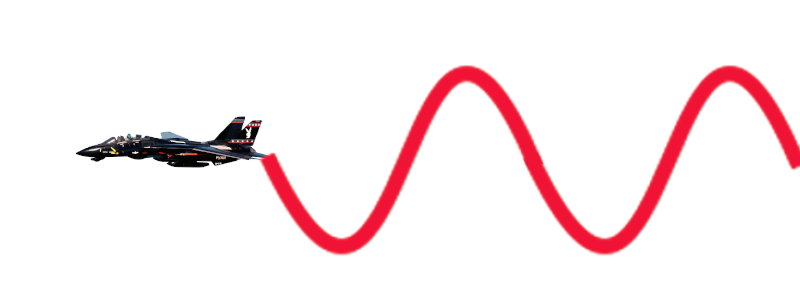
\includegraphics[scale=0.4]{Images/Enemy1-movement.png}
  \label{Bild 1}
  \caption{Hur Small plane rör sig åt vänster}
\end{figure}




\subsubsection*{Big plane}
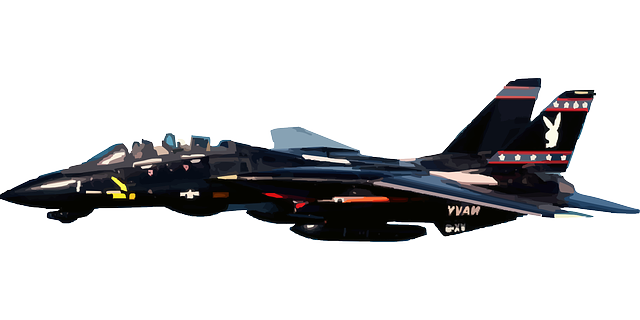
\includegraphics[scale=0.2]{Images/Enemy2.png}
\begin{itemize}
\item Den har en fixerad storlek, något större än Small plane.
\item Den har 2 liv.
\item Vid kollision skadar den spelaren med 2.
\item Den rör sig åt vänster enligt en linjärt mönster (se bild).
\item Den har röreslehastighet 2.
\item Den skjuter när den är i höjd med spelaren.
\end{itemize}
\begin{figure}[h!]
  \centering
  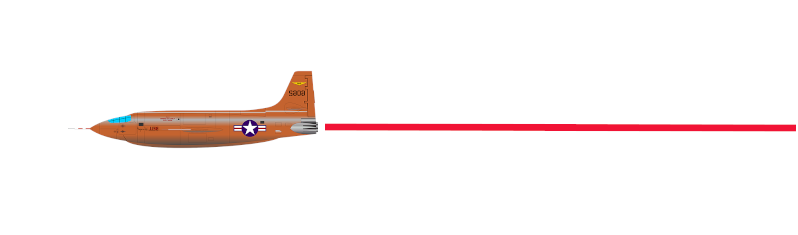
\includegraphics[scale=0.4]{Images/Enemy2-movement.png}
  \label{Bild 2}
  \caption{Hur Big plane rör sig åt vänster}
\end{figure}

\newpage
\subsubsection*{Bomb}
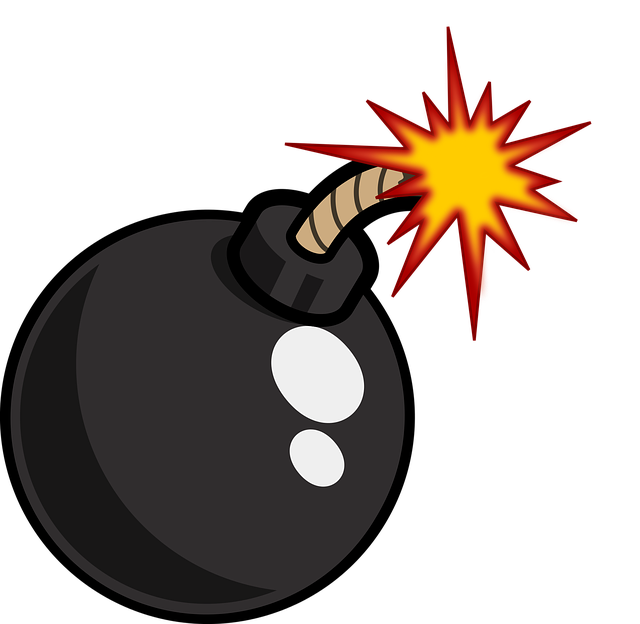
\includegraphics[scale=0.08]{Images/Bomb.png}\\
\begin{itemize}
\item De har en fixerad storlek, en bit mindre än spelaren.
\item Den har 1 liv.
\item Vid kollision skadar den spelaren med 1.
\item Den har rörelsehastighet 1.

\end{itemize}



\subsection{Power-up \& föremål}
Power-ups ger spelaren diverse positiva effekter när de plockas upp. De kommer in på spelplanen från höger sida och färdas åt vänster med hastighet 1. 
Power-ups plockas upp av spelaren då den kolliderar med dem. Alla power-ups har samma storlek.

\subsubsection*{Heal}
\begin{itemize}
\item Heal ökar spelarens liv med 1.
\item Spelaren kan inte få mer än tre liv.
\end{itemize}

\subsubsection*{Triple-shot}
\begin{itemize}
\item Triple-shot gör så att spelaren skjuter tre skott vid varje avfyrning istället för ett.
\item Denna varar 15 sekunder.
\item Om spelaren plockar upp en Triple-shot när den redan har effekten av en tidigare Triple-shot aktiv så återställs den kvarvarande tiden till 15 sekunder.
\end{itemize}

\subsubsection*{Shield}
\begin{itemize}
\item Shield Power-up gör spelaren odödlig i 10 sekunder.
\item Om spelaren plockar upp en Shield när den redan har effekten av en tidigare Shield aktiv så återställs den kvarvarande tiden till 10 sekunder.
\item Om spelaren kolliderar med en fiende och har shield-effekten aktiv så tas effekten bort och spelaren får samma odödlighetsperiod som om den hade tagit skada.  
\end{itemize}


\subsection{Poäng}
\begin{itemize}
\item Spelaren får 50 poöng när den förstör en bomb med sitt skott.
\item Spelaren får 100 poäng när den förstör ett fiende typ 1 med sitt skott.
\item Spelaren får 150 poäng när den förstör ett fiende typ 2 med sitt skott.
\item Spelaren förlorar 100 poäng ifall den kolliderar med en fiende.
\item Spelaren får 300 poäng om den plockar upp en Heal Power-up när den har redan fullt liv.
\item När slutet av en nivå har nåtts får spelaren stjärnor baserat på hur många poäng den samlade in av nivåns totala möjliga poäng.
\item 0-49\% ger en stjärna, 50-69\% ger två stjärnor, och 70-100\% ger tre stjärnor.
\end{itemize}

\section{Visualisering}
Det här är ett exempel på hur spelet kan se ut. Observera att spelaren är det vänstra flygplanet som pekar åt höger. Alla fiender och Power-ups rör sig åt höger enligt sitt mönster och hastighetsnivå. 

\begin{figure}[h!]
  \centering
  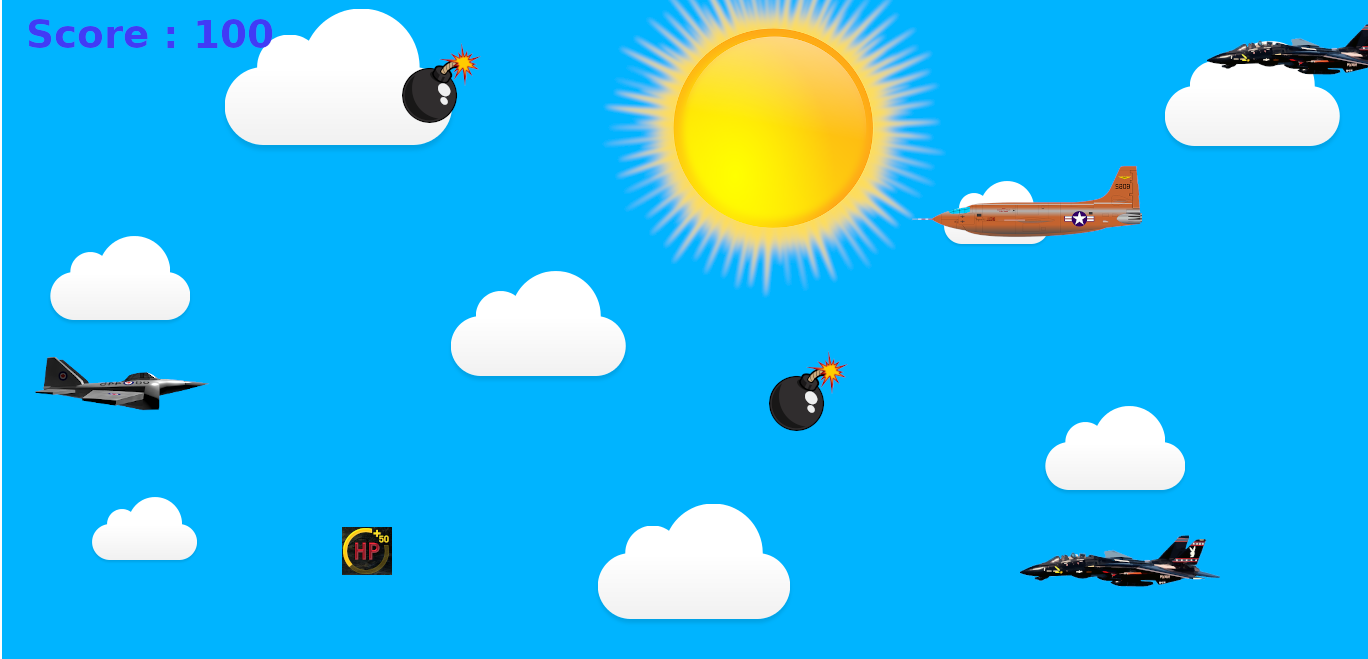
\includegraphics[scale=0.35]{Images/Game.png}
  \label{Bild 3}
  \caption{Ett exempel på hur en nivå kan se ut}
\end{figure}


\section{Krav}
Nedan kommer alla de krav som spelet i slutändan ska uppfylla. Ska-krav är högst prioriterade medan bör-krav ska uppfyllas om det finns tid över och kunskapen som krävs.

\subsection{Ska-krav}
\begin{enumerate}
\item Det ska finnas ett spelarobjekt.
\item Spelplanen ska ha en fixerad storlek som är lika stor som skärmen.
\item Spelet ska utspela sig i en 2D-miljö sedd från sidoperspektiv.
\item Spelet ska ha en startmeny där en nivå kan väljas, spelet kan avslutas, och hjälpsidan visas.
\item Spelet ska ha en hjälpsida där regler och kontroller förklaras.
\item Alla spelobjekt som visas på spelplanen ska ha en av 4 hastigheter som bestäms av vilken typ av objekt det är.
\item Spelaren ska kontrollera en spelarkaraktär.
\item Spelaren ska kunna röra på sig i åtta riktningar.
\item Spelaren ska ej kunna röra sig utanför spelplanens kanter
\item Spelaren styrs via tangentbordet. %10
\item Spelaren ska kunna skjuta skott framför sig.
\item Spelaren ska kunna förstöra fiender med sina skott.
\item Spelaren ska ta skada ifall den kolliderar med fiender eller deras skott.
\item Vid kollison med spelaren ska fiender förstöras.
\item Spelaren ska förlora poäng vid kollision med fiende.
\item Spelaren ska samla poäng när den förstör en fiende.
\item Spelaren ska samla poäng när den plockar upp en Heal Power-up när den har fullt liv.
\item Spelarens liv och poäng ska konstant visas på skärmen under rundans gång.
\item Spelaren ska bli odödlig under en kort period när den tar skada.
\item Spelaren ska inte kunna inte förstöra fiender via kollision under odödlighetsperioden. %20
\item När spelaren dör ska rundan avslutas och spelaren ges möjlighet att spela igen eller gå tillbaka till startmenyn. 
\item Det ska finnas 3 typer av fiender.
\item Fiender ska röra på sig enligt förbestämda mönster och hastigheter.
\item Vissa fiender ska skjuta skott.
\item Fiender ska ignorera kollision med andra fienders skott och modeller.
\item Fiender ska skada spelaren antingen genom att träffa den med skott eller genom att kollidera med den.
\item Fiender ska endast skjuta när de befinner sig i höjd med spelaren.
\item Det ska finnas en nivå (Level 1) i spelet.
\item Det ska kunna läggas till flera nivåer med använder samma spelobjekt.
\item Det ska kunna finnas flera fiender av samma typ på spelplanen samtidigt. %30
\item Fienderna ska röra på sig enligt ett mönster i spel nivån.
\item Det ska finnas tre olika power-ups som regelbundet färdas åt vänster över spelplanen.
\item Heal ska ge spelaren liv.
\item Shield ska ge spelaren odödlighet.
\item Triple-shot ska ge spelaren två extra skott. 
\item Spelaren ska kunna plocka upp Power-ups genom att kollidera med dem.
\end{enumerate}

\subsection{Bör-krav}
\begin{enumerate}
\item Spelet ska ha ljud för diverse händelser.
\item Speler ska ha bakgrundsmusik.
\item Power-ups ska dras mot spelaren då den kommer i närheten av dem.
\item Antalet intjänade poäng ska sparas när spelaren till slut förlorar och rundan är avslutad.
\item Spelet ska ha en sida där intjänade poäng från tidigare rundor visas i en topplista.
\item Spelet ska ha en sida där användaren kan ändra vilka tangenter som gör vad.
\item Bakgrunden ska röra på sig för att ge användaren en känsla av hastighet.
\item Spelet ska ha fler nivåer utöver den första.
\item Spelaren ska få en diamant-stjärna ifall den klarar av en nivå med 100\% av alla möjliga poäng.
\item Det ska finnas fusk-kommandon som ger enorma bonusar.
\item Fiender ska ha en chans att släppa ifrån sig power-ups när de förstörs av spelaren.

\end{enumerate}

\section{Kravuppfyllelse}
\textit{\textbf{``Spelet ska simulera en värld som innehåller olika typer av objekt. Objekten ska ha olika beteenden och röra sig i världen och agera på olika sätt när de möter andra objekt.''}}


Uppfylls av krav 3, 8, 12, 13, 14, 15, 22, 26\\


\textit{\textbf{``Det måste finnas minst tre olika typer av objekt och det ska finnas flera instanser av minst två av dessa. T.ex ett spelarobjekt och många instanser av två olika slags fiendeobjekt.''}}


Uppfylls av krav 1, 22, 32\\

\textit{\textbf{``Ett beteende som måste finnas med är att figurerna ska röra sig över skärmen. Rörelsen kan följa ett mönster och/eller vara slumpmässig. Minst ett objekt, utöver spelaren ska ha någon typ av rörelse.''}}


Uppfylls av krav 23 och 32\\

\textit{\textbf{``En figur ska styras av spelaren, antingen med tangentbordet eller med musen. Du kan även göra ett spel där man spelar två stycken genom att dela på tangentbordet (varje spelare använder olika tangenter). Då styr man var sin figur.''}}


Uppfylls av krav 7 och 8\\

\textit{\textbf{``Grafiken ska vara tvådimensionell.''}}


Uppfylls av krav 3\\

\textit{\textbf{``Världen (spelplanen) kan antas vara lika stor som fönstret ''}}


Uppfylls av krav 2\\

\textit{\textbf{``Det ska finnas kollisionshantering, det vill säga, det ska hända olika saker när objekten möter varandra, de ska påverka varandra på något sätt. T.ex kan ett av objekten tas bort, eller så kan objekten förvandlas på något sätt, eller så kan ett nytt objekt skapas. ''}}


Uppfylls av krav 12, 13, 14, 15, 26, 36\\

\textit{\textbf{``Det ska vara enkelt att lägga till eller ändra banor i spelet. Detta kan exempelvis lösas genom att läsa in banor från en fil, eller genom att ha funktioner i programkoden som bygger upp en datastruktur som definierar en  nivå .''}}


Uppfylls av 29\\

\textit{\textbf{`` Spelet måste upplevas som ett sammanhängande spel som går att spela! ''}}

Ska uppfyllas av alla ska-krav tillsammans.

\end{document}

